\begin{frame}
\titlepage
\end{frame}
\begin{frame}{This lecture}
\vspace*{1cm}
\begin{itemize}
\item training as optimization
\item backpropagation
\item language modeling
\end{itemize}
\end{frame}
%%%%%%%%%%%%%%%%%%%%%%%%%%%%%%%%
\begin{frame}{Recall}
    \begin{itemize}
        \item<1-> the input to a supervised learning algorithm is a training set ($x_{1:n}, y_{1:n}$), where
        \begin{itemize}
            \item<2-> $x_{1:n} = x_1,x_2,..., x_n$ shows input examples
            \item<3->  $y_{a:n}= y_1, y_2, ..., y_n$ shows corresponding labels
        \end{itemize}
        \item<4-> the goal of a learning algorithm is to return a function $f()$ that accurately maps input examples to their desired labels
        \uncover<5->{
        \begin{figure}
\centering
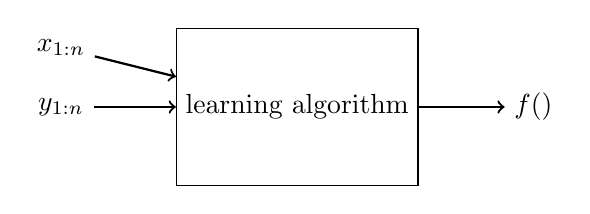
\begin{tikzpicture}

\node(x) at (0, 0) [] {$x_{1:n}$};
\node(y) at (0, -0.75) [] {$y_{1:n}$};


\node(lr) at (3,-0.75) [draw, minimum width=2cm, minimum height=2cm]{learning algorithm};

\draw[->,thick] (x) to (lr);
\draw[->,thick] (y) to (lr);

\node(f) at (6.0, -0.75) [] {$f()$};
\draw[->,thick] (lr) to (f);

\end{tikzpicture}
\end{figure}
        }
        \item<6-> how to measure if $f()$ works accurately?  
    \end{itemize}
\end{frame}
\begin{frame}{Loss Function}
\begin{itemize}
    \item<1->  \emph{Loss function $L(y,\hat{y})$}: It quantifies the loss suffered when predicting $\hat{\mathbf{y}}$ while the true label is $\mathbf{y}$
    
    \item<2-> given a labeled training set $(x_{1:n};y_{1:n})$, a per-instance loss function $L$ and a parameterized function $f(x;\Theta)$, we define the corpus-wide loss with respect to the parameters‚ as the average loss over all training examples:
    \begin{equation*}
        \mathcal{L}(\theta) = \frac{1}{n}\sum_{i=1}^{n}L(\hat{y},y_i),
    \end{equation*}
        \begin{equation*}
        \hat{y} = f(x_i;\Theta)
    \end{equation*}
\item<3-> in this view the training examples are fixed and the values of the parameters determine the loss
\end{itemize}
\end{frame}
\begin{frame}{Training as Optimization}
    \begin{itemize}
        \item<1-> the goal of the training algorithm is then to set the values of the parameters such that the value of $\mathcal{L}$ is minimized
        \begin{equation*}
            \hat{\Theta} = \text{argmin}_{\Theta} \mathcal{L}(\Theta) =\text{argmin}_{\Theta} \frac{1}{n}\sum_{i=1}^{n}L(\hat{y},y_i) 
        \end{equation*}
      \end{itemize}
\end{frame}
\begin{frame}{Common Loss Functions}
    \begin{itemize}
        \item Hinge (binary)
        \begin{itemize}
            \item<1-> for binary classification problems
            \item<2-> the classifier’s output is a single scalar $\hat{y}$ and the true output $y$ is in $\{-1,+1\}$
            \item<3-> the inference rule is prediction$= \text{sign}(\hat{y})$, and a classification is considered correct if $y \cdot \tilde{y} > 0$ 
            \item<4-> per-instance loss:
            \begin{equation*}
              L_{\text{hinge(binary)}} (\hat{y}, y) = \text{max}(0, 1 - y. \hat{y}) 
            \end{equation*}
        \end{itemize}
    \end{itemize}
\end{frame}
\begin{frame}{Common Loss Functions}
    \begin{itemize}
        \item Hinge (multi-class)
        \begin{itemize}
            \item<1-> let $\hat{y} =  \hat{y}_{[1]},\hat{y}_{[2]},..., \hat{y}_{[n]} $ be the model’s output vector, and $y$ be the one-hot vector for the correct output class
            \item<2-> the inference rule is defined as selecting the class with the highest score
             $\text{prediction}= \text{argmax}_{i}\hat{y}_{[i]}$
             \item<3-> if $t$ is the correct class and $k$ is the highest scoring class such that $k \neq t$ then loss is
                \begin{equation*}
              L_{\text{hinge(multiclass)}} (\hat{y}, y) = \text{max}(0, 1- (\hat{y}_{[t]}-\hat{y}_{[k]}))
            \end{equation*}
        \end{itemize}
    \end{itemize}
\end{frame}
\begin{frame}{Common Loss Functions}
    \begin{itemize}
        \item Log loss
        \begin{itemize}
            \item<1-> can be seen as a ``soft'' version of the hinge loss with an infinite margin 
             \item<2-> loss
                \begin{equation*}
              L_{\text{log}} (\hat{y}, y) = \text{log}(1+\text{exp}(-(\hat{y}_{[t]}-\hat{y}_{[k]}))
            \end{equation*}
        \end{itemize}
    \end{itemize}
\end{frame}
\begin{frame}{Common Loss Functions}
    \begin{itemize}
        \item<1-> binary cross entropy (logistic loss)
        \begin{itemize}
            \item<2-> used for binary classification with conditional probability outputs. 
            \item<3-> assumes a set of two target classes labeled 0 and 1, with a correct label $y\in \{0, 1\}$
            \item<4-> the model’s output $\tilde{y}$ is transformed using the sigmoid function
            \begin{equation*}
                \sigma(x) = \frac{1}{1+e^{-x}}
            \end{equation*}
            \item<5-> then $\hat{y} = \sigma(\tilde{y}) = P(y=1|x)$
            \item<6-> inference rule: prediction$=0$ if $\hat{y}<0.5$ and prediction$=1$ if $\hat{y}>=0.5$
             \item<7-> loss
                \begin{equation*}
              L_{\text{logistic}} (\hat{y}, y) = -y\text{log}(\hat{y}) -(1-y)log(1-\hat{y})
            \end{equation*}
            \item<8->  is useful for estimating class conditional probability for a binary classification problem
            \item<9-> we assume that the output layer is transformed using sigmoid
        \end{itemize}
    \end{itemize}
\end{frame}
\begin{frame}{Training as Optimization}
    \begin{itemize}
        \item<1-> the goal of the training algorithm is then to set the values of the parameters such that the value of $\mathcal{L}$ is minimized
        \begin{equation*}
            \hat{\Theta} = \text{argmin}_{\Theta} \mathcal{L}(\Theta) =\text{argmin}_{\Theta} \frac{1}{n}\sum_{i=1}^{n}L(\hat{y},y_i) 
        \end{equation*}
      \item<2-> the above optimization attempts to minimize the loss at all costs, which may result in overfitting the training data 
      \end{itemize}
\end{frame}
\begin{frame}{Regularization}
    \begin{itemize}
     
        \item<1-> to counter that we define a regularization term $R(\Theta)$ taking as input the parameters and returning a scalar that reflect their ``complexity,'' which we want to keep low
        
        \item<2-> training 
        \begin{equation*}
            \hat{\Theta} = \text{argmin}_{\Theta} \mathcal{L}(\Theta) =\text{argmin}_{\Theta} \frac{1}{n}\sum_{i=1}^{n}L(\hat{y},y_i) 
        \end{equation*}
     
     \item<3-> training with regularization
        \begin{equation*}
            \hat{\Theta} = \text{argmin}_{\Theta} \mathcal{L}(\Theta) =\text{argmin}_{\Theta} \left( \frac{1}{n}\sum_{i=1}^{n}L(\hat{y},y_i)  + \lambda R(\Theta) \right)
        \end{equation*}
    \end{itemize}
\end{frame}
\begin{frame}{Regularization}
    \begin{itemize}
        \item<1-> intuitively we would like to drive the learner toward natural solutions, in which it is OK to mis-classify a few examples if they don’t fit well with the rest
        \begin{equation*}
            \hat{\Theta} =\text{argmin}_{\Theta} \left( \frac{1}{n}\sum_{i=1}^{n}L(\hat{y},y_i)  + \lambda R(\Theta) \right)
        \end{equation*}
        \item<2-> regularization term considers the parameter values, and scores their complexity
        \item<3-> in practice the regularizers equate complexity with large weights and work to keep the parameter values low 
        
    \end{itemize}
\end{frame}
\begin{frame}{Common Regularization Functions}
    \begin{itemize}
        \item<1-> $L_2$ regularization (a.k.a. gaussian prior or weight decay): It keeps the sum of the squares of the parameter values low
        \begin{equation*}
            R_{L_2}(W) = ||W||_2^2 = \sum_{i,j}{(W_{[i,j]})^2}
        \end{equation*}
        \item<2-> the learner will prefer to decrease the value of one parameter with high weight by $1$ than to decrease the value of ten parameters that already have relatively low weights by $0.1$ each
    \end{itemize}
\end{frame}
\begin{frame}{Common Regularization Functions}
    \begin{itemize}
        \item<1-> $L_1$ regularization (a.k.a. sparse prior or lasso): It keeps  the sum of the absolute values of the parameters low
        \begin{equation*}
            R_{L_1}(W) = ||W||_1 = \sum_{i,j}{|W_{[i,j]}|}
        \end{equation*}
        \item<2-> the learner will prefer to decrease all the non-zero parameter values toward zero
    \end{itemize}
\end{frame}
\begin{frame}{Common Regularization Functions}
    \begin{itemize}
        \item<1-> Elastic-Net: combines both $L_1$ and $L_2$ regularization
        \begin{equation*}
            R_{\text{elastic-net}}(W) = \gamma_1 R_{L_1}(W) + \gamma_2 R_{L_2}(W)
        \end{equation*}
        \item<2-> dropout: will be discussed later
    \end{itemize}
\end{frame}
\begin{frame}{Training as Optimization}
    \begin{itemize}
        \item<1-> we learned that the goal of training is to minimize a loss function (and a regularization term)
        \begin{equation*}
            \hat{\Theta} =\text{argmin}_{\Theta} \left( \mathcal{L}(\hat{y},y)  + \lambda R(\Theta) \right)
        \end{equation*}
        \item<2-> training = Solving an optimization problem
        \item<3-> how to find parameter values that minimize loss?
    \end{itemize}
\end{frame}
\begin{frame}{Gradient-based Optimization}
   
  \only<1-1>{
    \begin{figure}
        \centering
        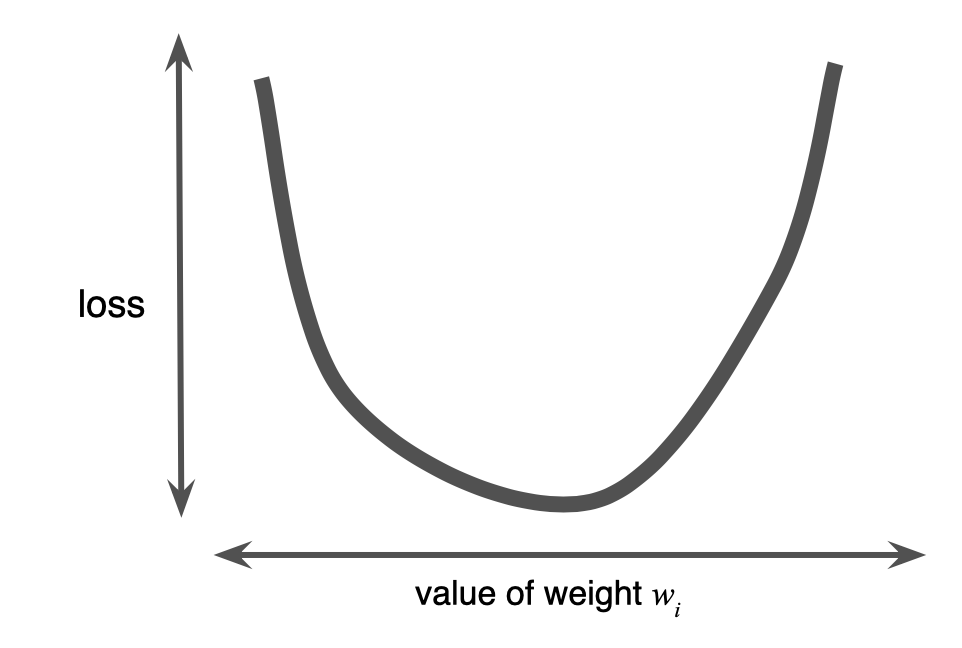
\includegraphics[scale=0.2]{final/lecture03/figures/sgd1.png}
    \end{figure}
    }
    \only<2-2>{
        \begin{figure}
        \centering
        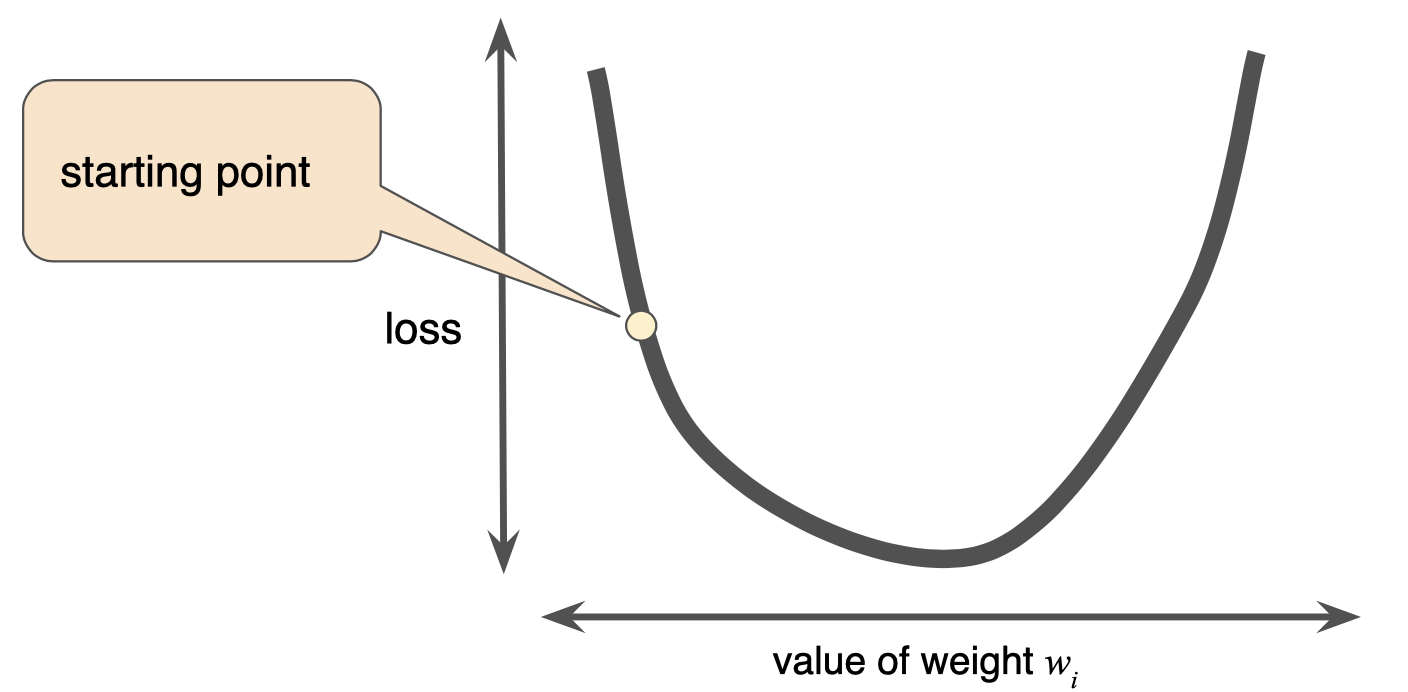
\includegraphics[scale=0.2]{final/lecture03/figures/sgd2.png}
    \end{figure}
    }
    \only<3-3>
    {
      \begin{figure}
        \centering
        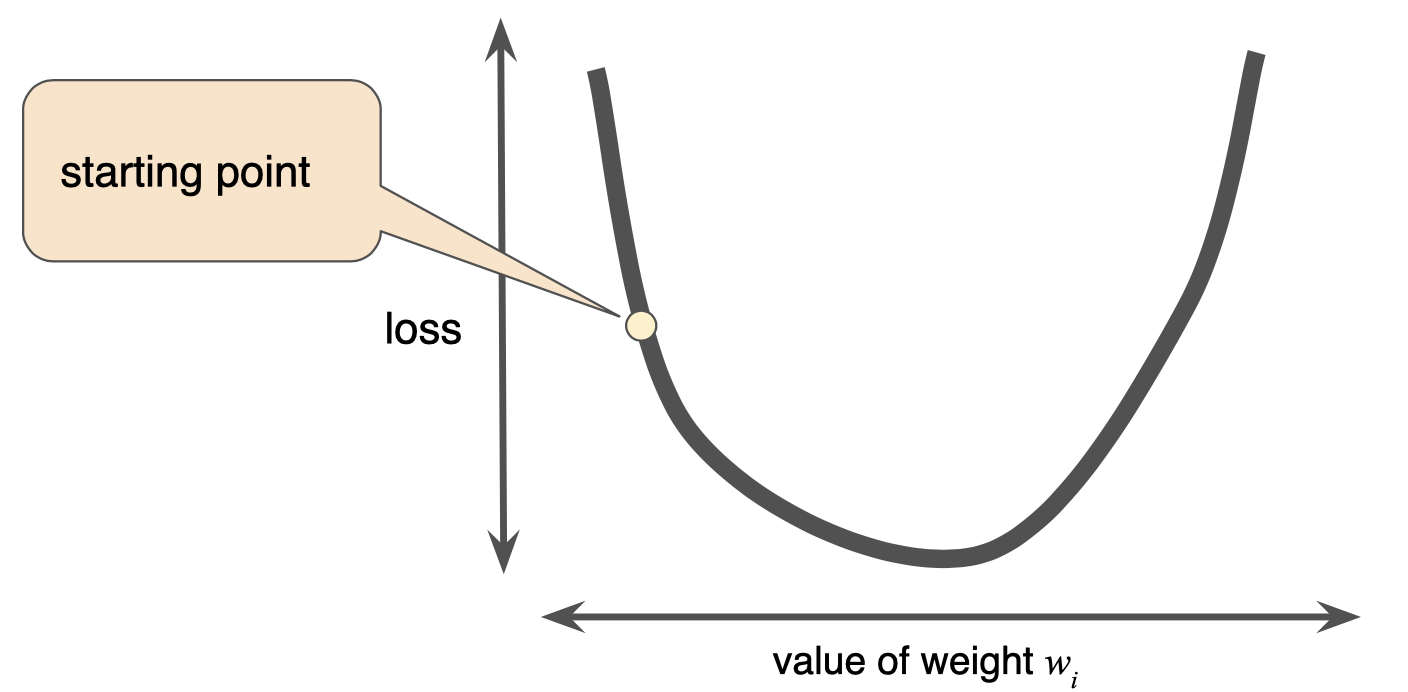
\includegraphics[scale=0.2]{final/lecture03/figures/sgd2.png}
    \end{figure}      
    }
    \only<4-4>
    {
     \begin{figure}
        \centering
        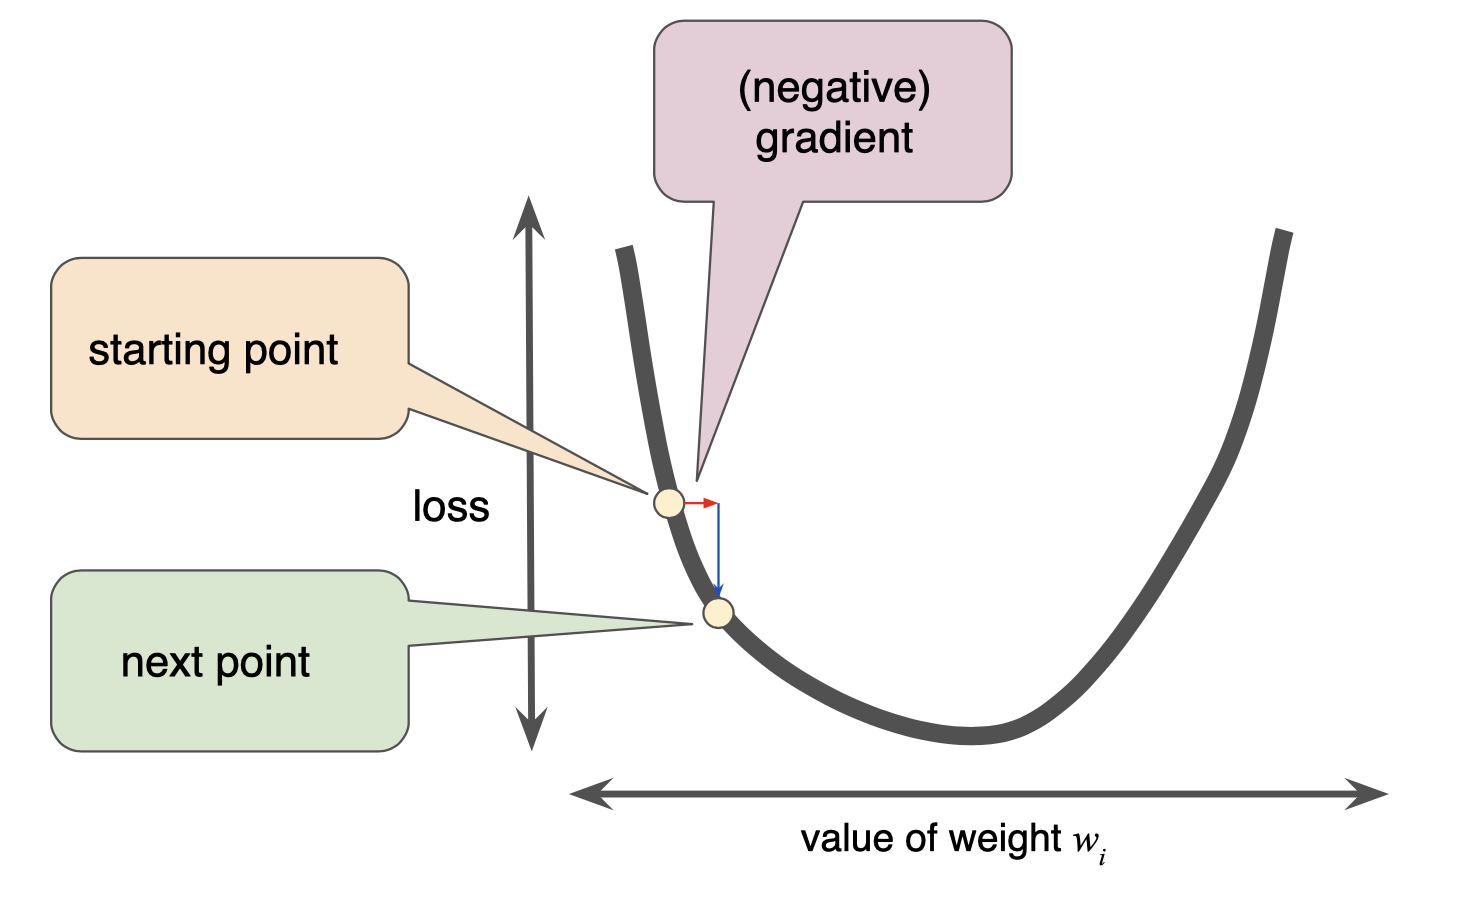
\includegraphics[scale=0.2]{final/lecture03/figures/sgd4.png}
    \end{figure}
    }
\vspace*{\fill}
\textit{\tiny{(Taken from: 
\url{https://developers.google.com/machine-learning/crash-course/reducing-loss/gradient-descent})}}
   
\end{frame}
\begin{frame}{Gradient-based Optimization}
    \begin{itemize}
        \item<1-> we repeatedly compute an estimate of the loss over the training set
        \item<2-> we compute the gradients of the parameters with respect to the loss estimate
        \item<3-> we move the parameter values in the opposite directions of the gradient
    \end{itemize}
\end{frame}
\begin{frame}{(Online) Stochastic Gradient Descent}
\centering
\begin{figure}
    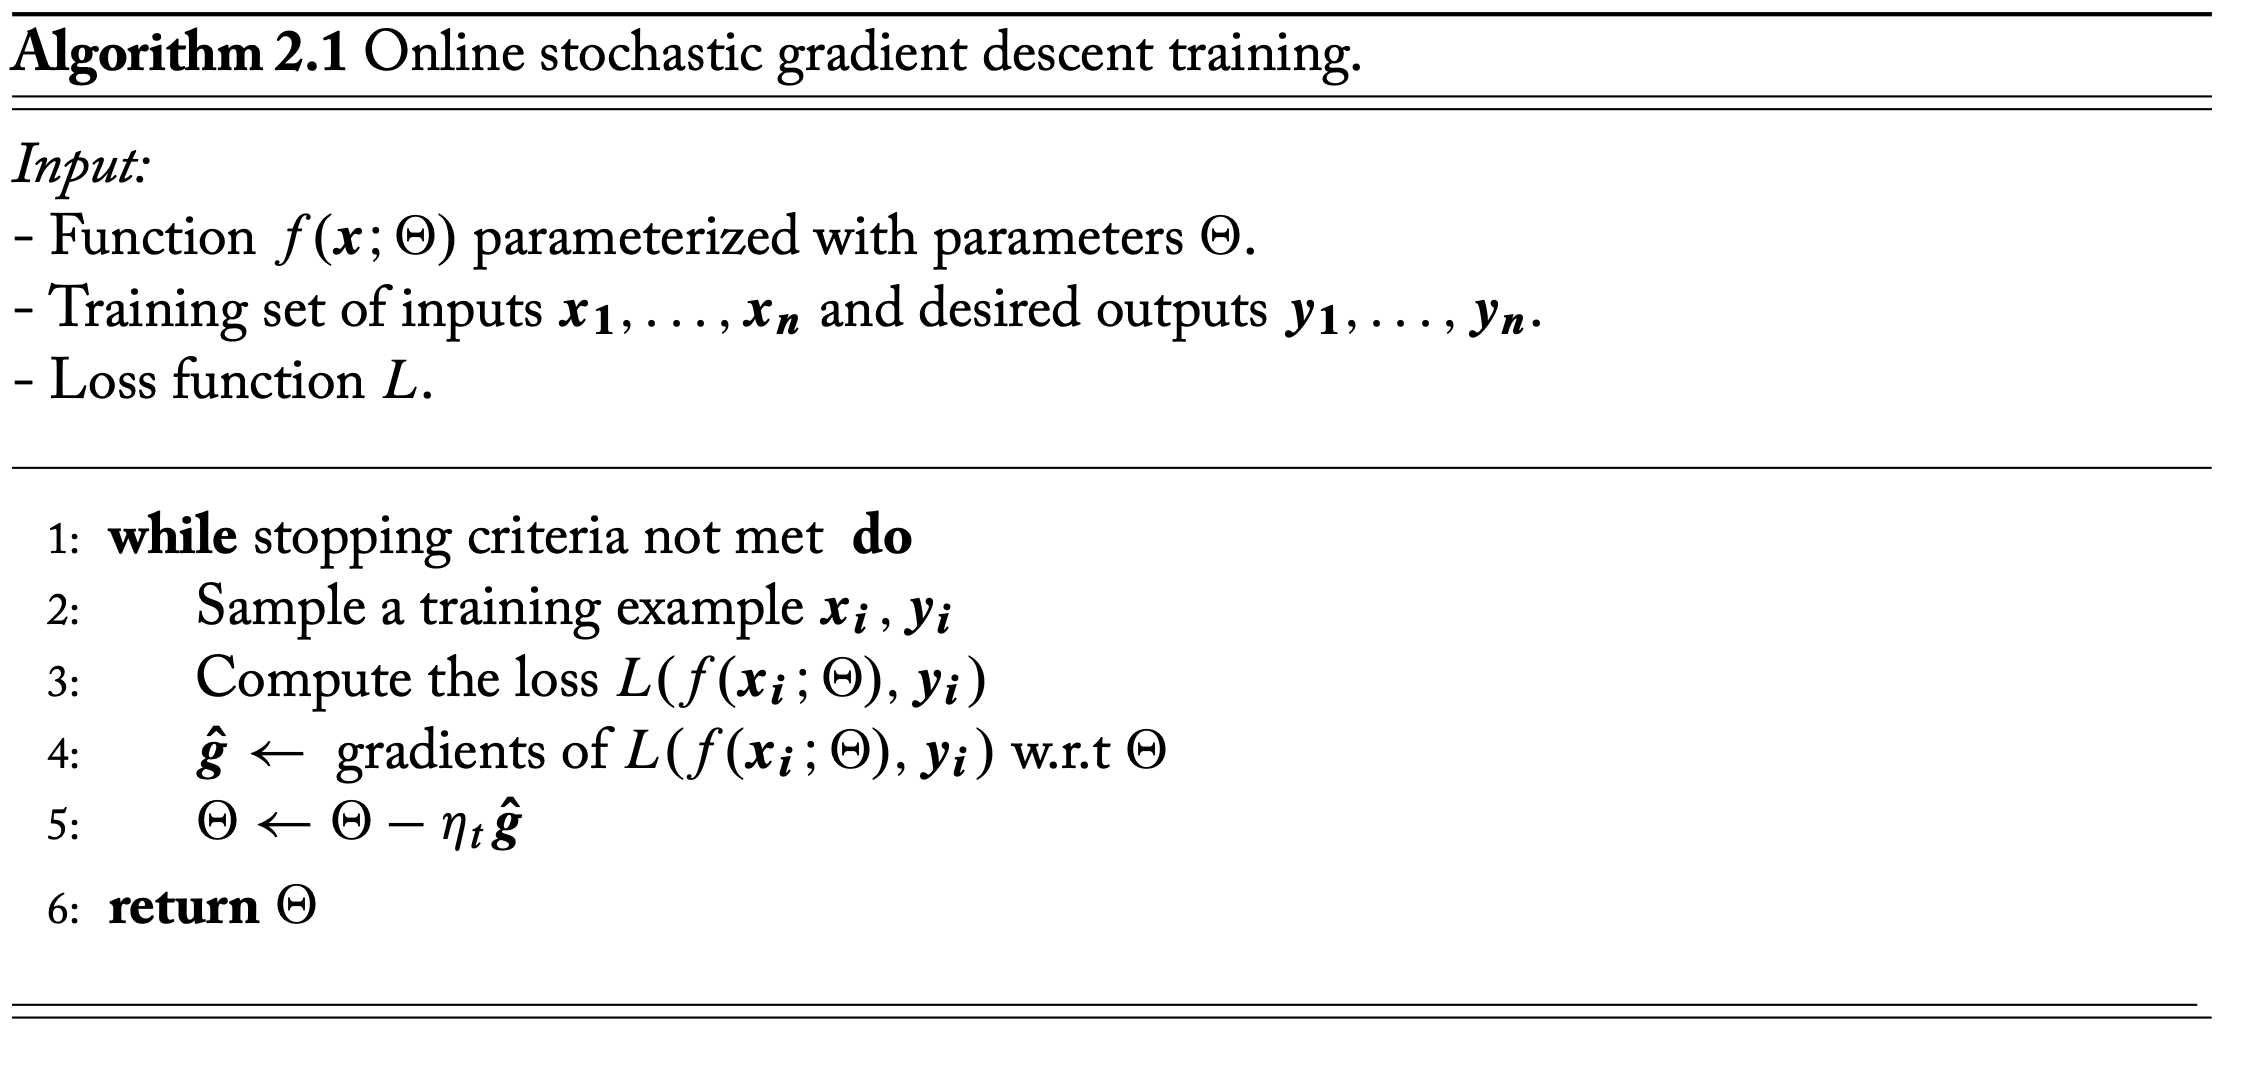
\includegraphics[scale=0.25]{final/lecture03/figures/sgd.png}
\end{figure}
\vspace*{\fill}
\textit{\tiny{(Taken from: Neural Network Methods for Natural Language Processing, Yoav Goldberg)}}
\end{frame}
\begin{frame}{\Large{(Minibatch) Stochastic Gradient Descent}}
\centering
\begin{figure}
    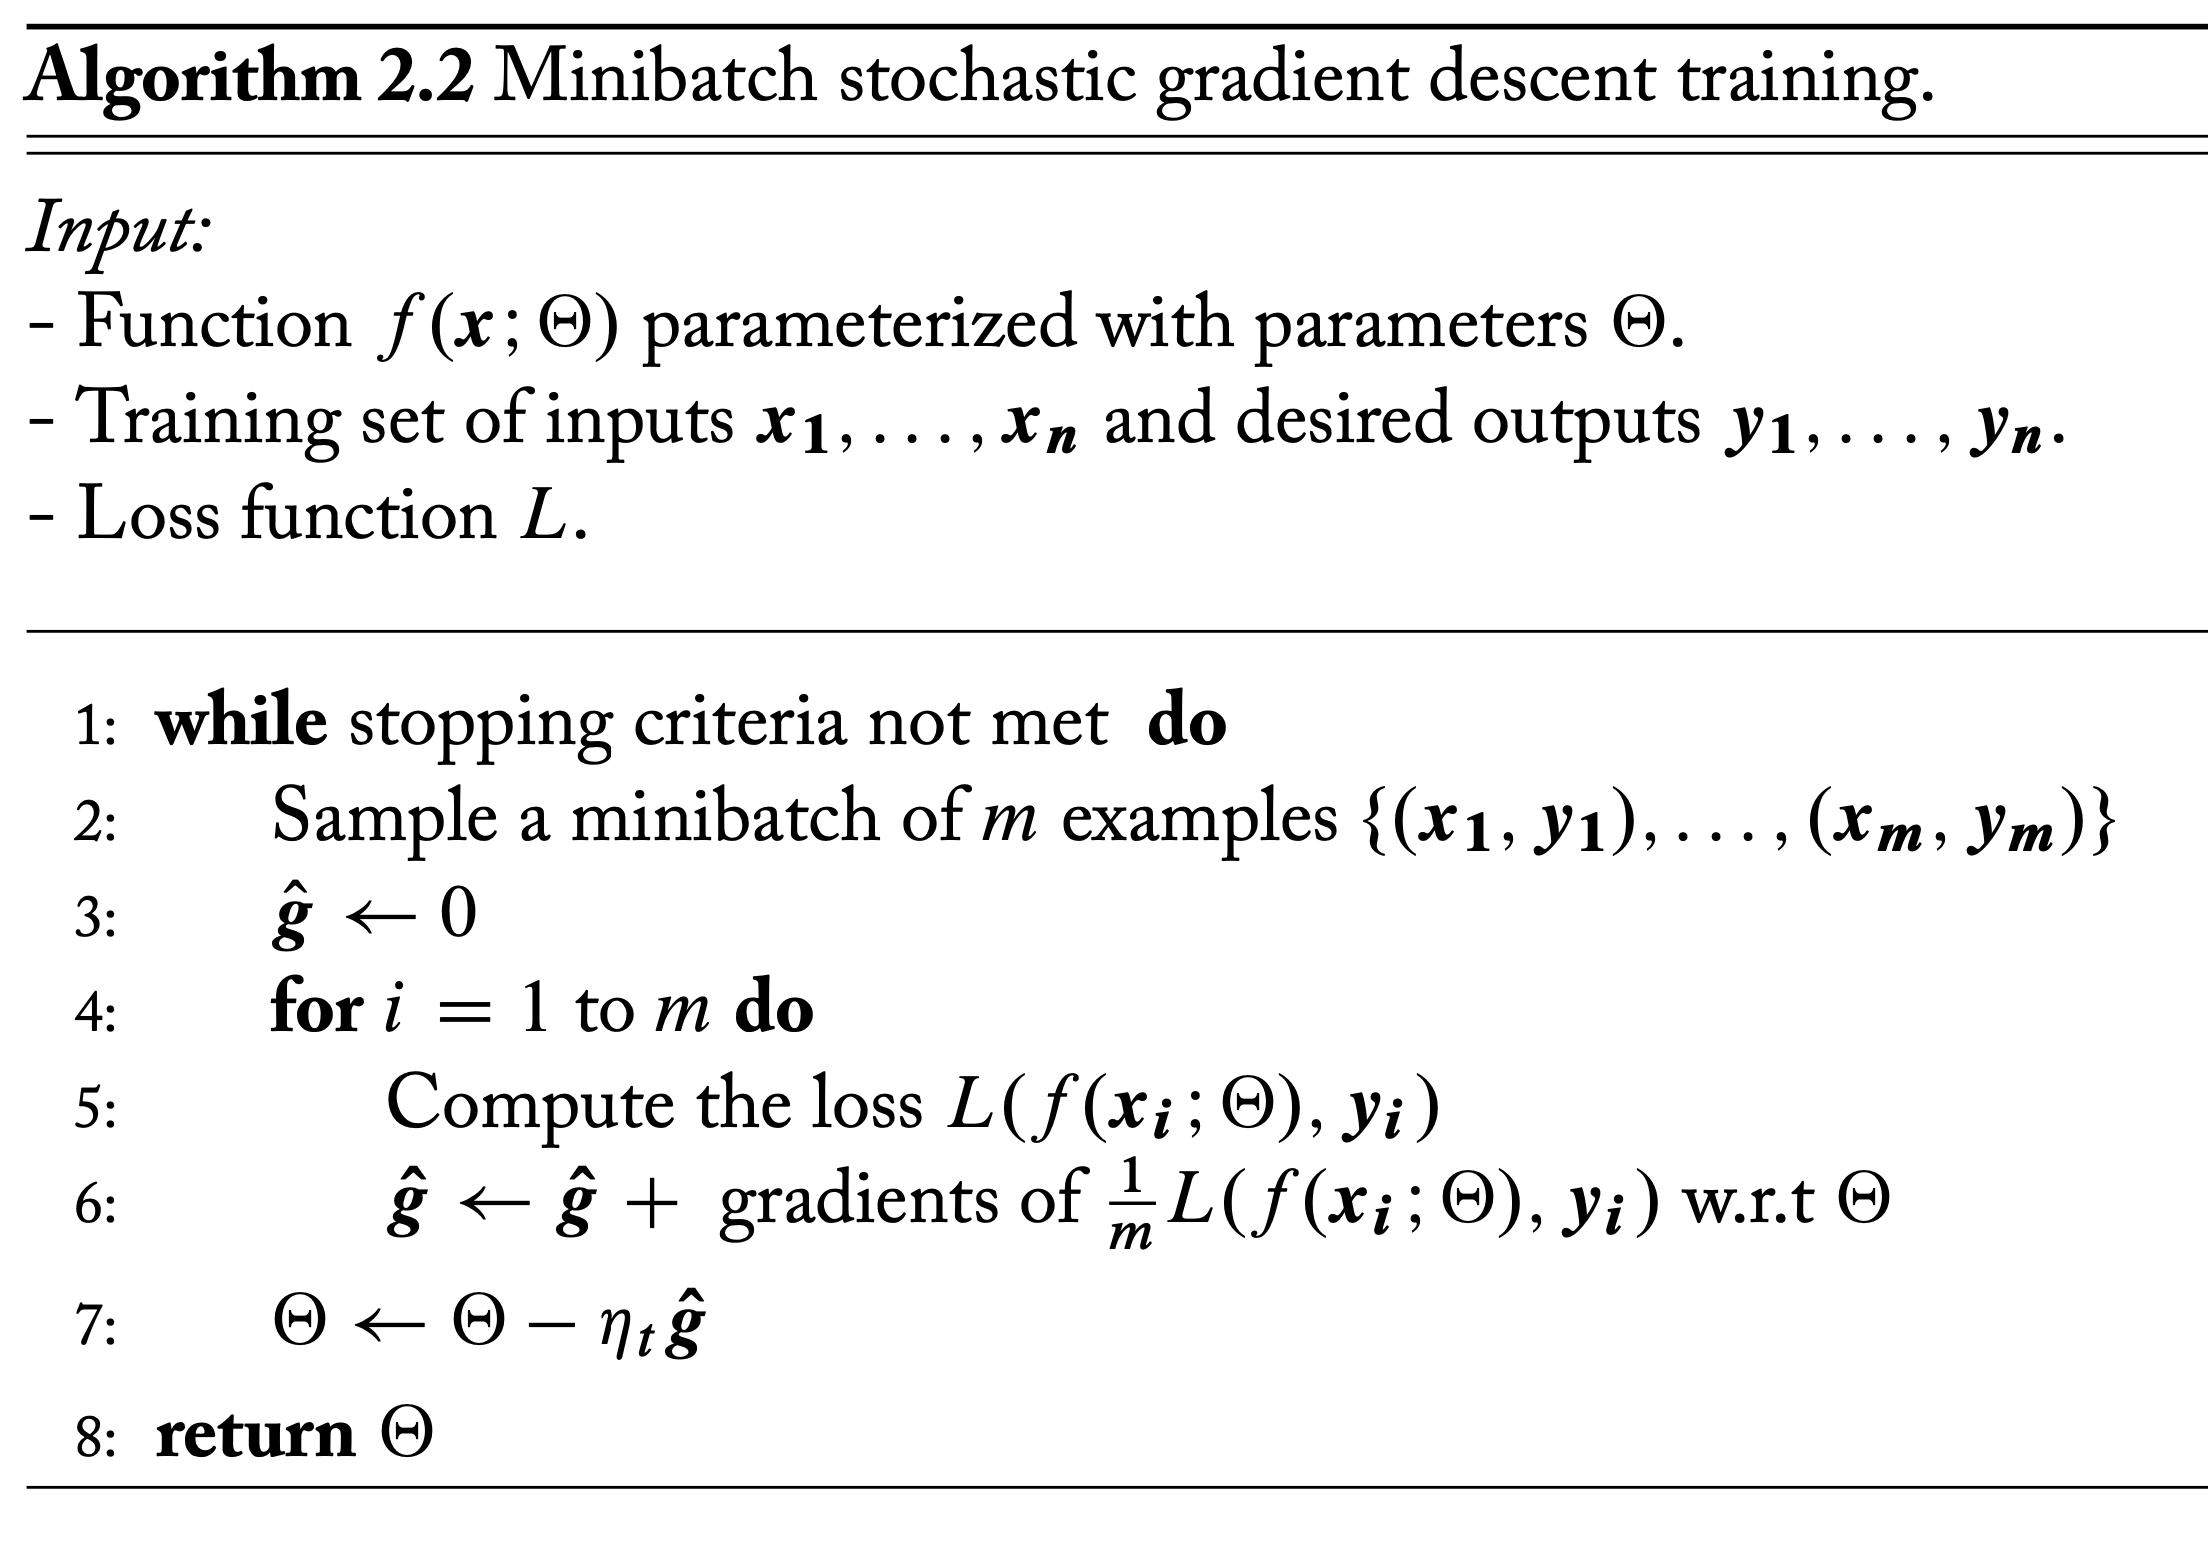
\includegraphics[scale=0.20]{final/lecture03/figures/msgd.png}
\end{figure}
\vspace*{\fill}
\textit{\tiny{(Taken from: Neural Network Methods for Natural Language Processing, Yoav Goldberg)}}
\end{frame}
\begin{frame}{Why Minibatch SGD?}
    \begin{itemize}
        \item<1-> it's not expensive: while computing loss function gradient on all training set can be computationally
expensive 
        \item<2-> it converges faster to a good solution than full-batch learning, in which we use all training set to compute gradient
        \item<3-> smaller mini-batch sizes lead often to better solutions (generalize better)
    \end{itemize}
\end{frame}
\begin{frame}{Stochastic Gradient Descent (SGD)}
    \begin{itemize}
        \item<1-> gradient descent does not always lead to best solutions
        \begin{figure}
            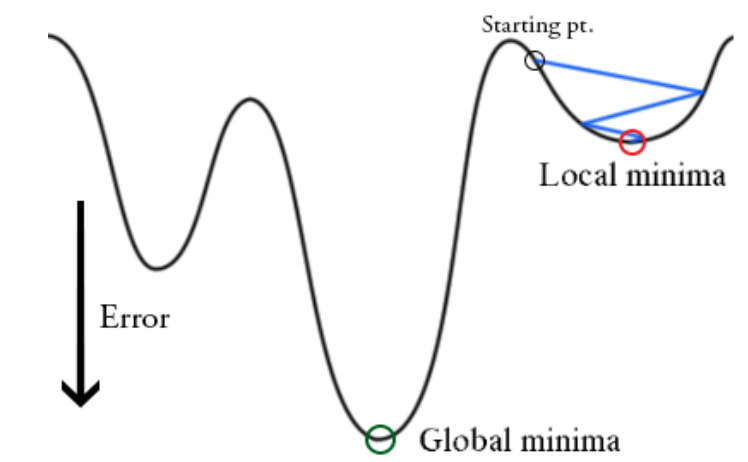
\includegraphics[scale=0.3]{final/lecture03/figures/sgd5.png}
        \end{figure}
        \item<2-> why? 
        \item<3-> SGD is sensitive to the learning rate and initial parameter values (starting point)
    \end{itemize}
\end{frame}
\begin{frame}{Small Learning Rate}
         \begin{figure}
        \centering
         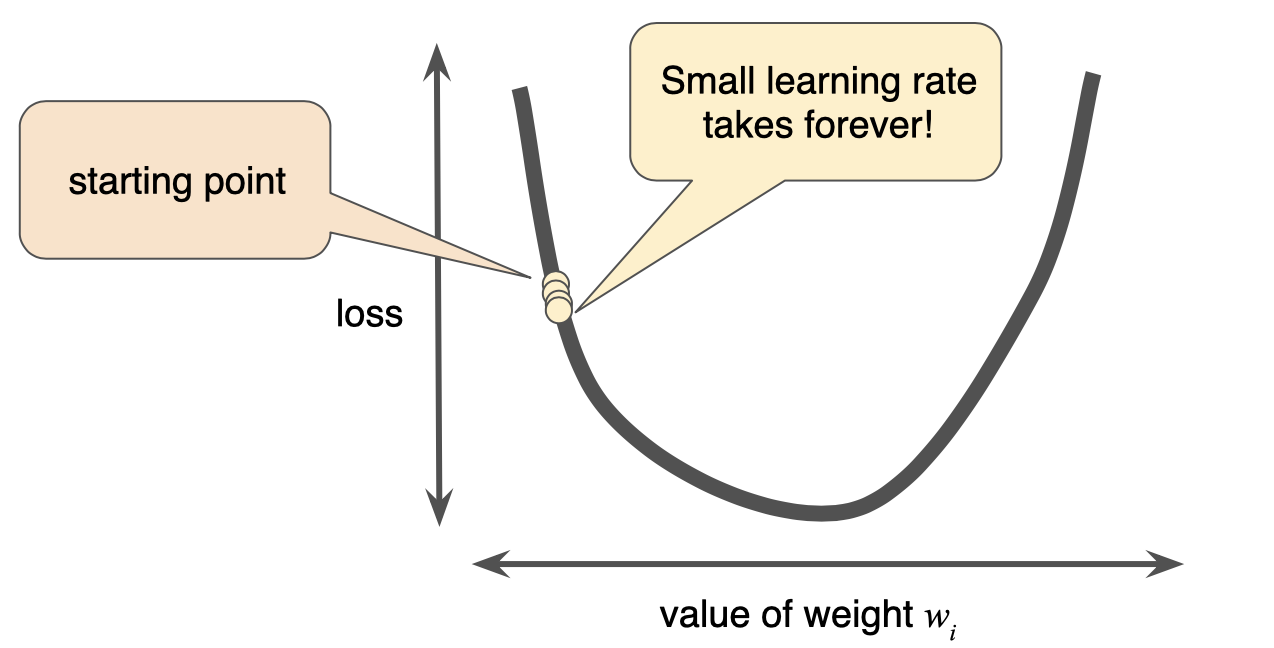
\includegraphics[scale=0.4]{final/lecture03/figures/small_lr.png}
        \end{figure}
\vspace*{\fill}
\textit{\tiny{(Taken from: 
\url{https://developers.google.com/machine-learning/crash-course/reducing-loss/gradient-descent})}}     
\end{frame}
\begin{frame}{Large Learning Rate}
         \begin{figure}
        \centering
          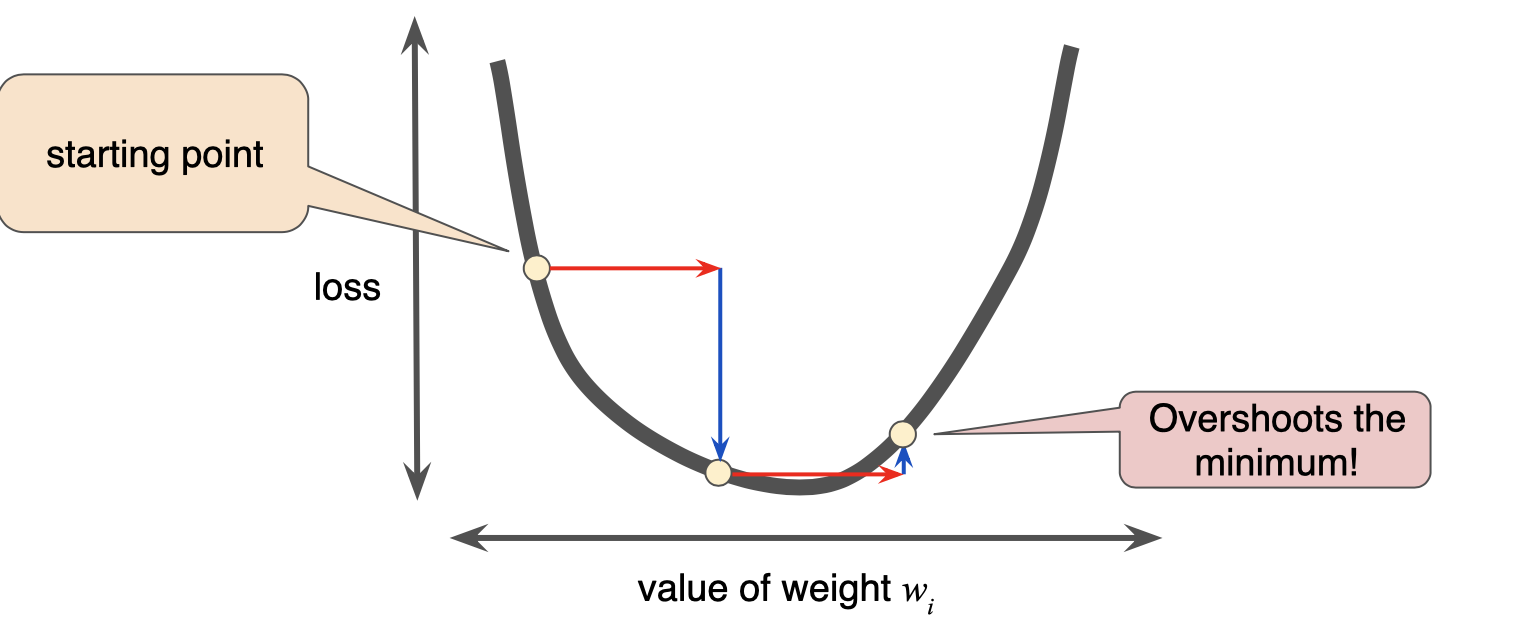
\includegraphics[scale=0.4]{final/lecture03/figures/large_lr.png}
        \end{figure}
\vspace*{\fill}
\textit{\tiny{(Taken from: 
\url{https://developers.google.com/machine-learning/crash-course/reducing-loss/gradient-descent})}}
\end{frame}
\begin{frame}{Adaptive Learning Rate}
         \begin{figure}
        \centering
        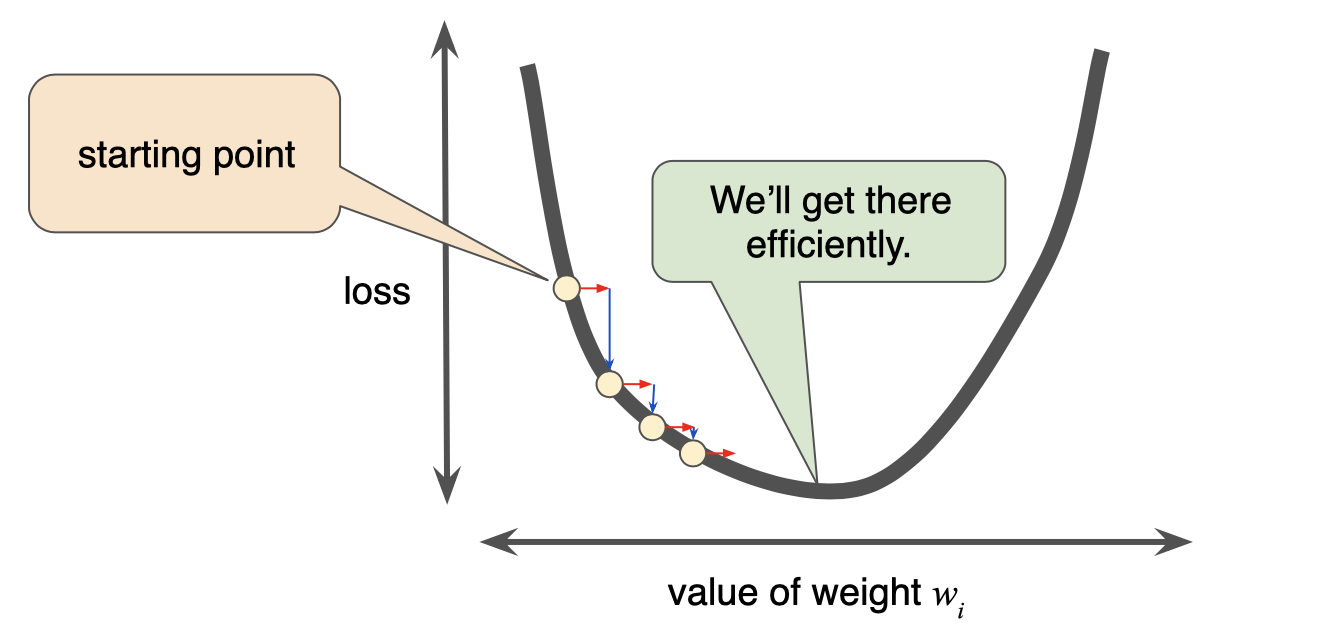
\includegraphics[scale=0.40]{final/lecture03/figures/adaptive_lr.png}
        \end{figure}
\vspace*{\fill}
\textit{\tiny{(Taken from: 
\url{https://developers.google.com/machine-learning/crash-course/reducing-loss/gradient-descent})}}
\end{frame}
\begin{frame}{Stochastic Gradient Descent (SGD)}
    \begin{itemize}
        \item<1-> Use adaptive learning rate algorithms 
        \begin{itemize}
            \item<1->  AdaGrad [Duchi et al., 2011], 
            \item<1-> AdaDelta [Zeiler, 2012], 
            \item<1-> RMSProp [Tieleman and Hinton, 2012], 
            \item<1-> Adam [Kingma and Ba, 2014] 
        \end{itemize}
        \item<2-> these methods train usually faster than SGD
        \item<3-> found solution is often not as good as that by SGD $\rightarrow$ First train with Adam, fine-tune with SGD
        \item<4-> they use different initial parameter values in different runs of experiments and report the average of scores
    \end{itemize}
\end{frame}
\begin{frame}{Backpropagation}
\begin{itemize}
    \item<1-> a fancy name for a recursive algorithm that computes the derivatives of a nested functions using the chain rule, while caching intermediary derivatives 
    \item<2-> chain rule: Assume $y = f(g(x))$
    \begin{equation*}
        \frac{\partial y}{\partial x} = \frac{\partial f}{\partial g}\times \frac{\partial g}{\partial x}   = \frac{\partial f}{\partial g}\frac{\partial g}{\partial x}
    \end{equation*}
\end{itemize}
\end{frame}
\begin{frame}{Backpropagation}
\begin{itemize}
    \item<1-> consists of two steps
    \begin{itemize}
        \item<2-> forward pass $\rightarrow$ use current parameter values to compute the loss value
        \item<3-> backward pass $\rightarrow$ use the gradient of the loss to update the parameter values
    \end{itemize}
\end{itemize}
\end{frame}

\begin{frame}{Model: Multilayer Perceptron (MLP) }
    \centering
    \scalebox{0.5}{
        \begin{tikzpicture}
        \uncover<1->{
        \node[] (x) at (0,0) {$x$};
        \node[draw, minimum height=2, minimum width=3] (l1) at (0,1) {$ f \left( x W^{(1)} \right) $};
        \draw[->, thick] (x) -- (l1);
        
         \node[] (h1) at (0,4) {$h^{(1)}$}; 
        \draw[->, thick] (l1) -- (h1);
        
        \node[draw, minimum height=2, minimum width=3] (l2) at (0,5) {$ f \left( h^{(1)} W^{(2)} \right) $};
        \draw[->, thick] (h1) -- (l2);
        
        
         \node[] (h2) at (0,8) {$h^{(2)}$}; 
        \draw[->, thick] (l2) -- (h2);
        
        \node[draw, minimum height=2, minimum width=3] (l3) at (0,9) {$ f \left( h^{(2)} W^{(3)} \right) $};
        \draw[->, thick] (h2) -- (l3);
        
        \node[] (y_hat) at (0,12) {$\hat{y}$}; 
        \draw[->, thick] (l3) -- (y_hat);
        
     \node[draw, white] (dummy-node) at (22,0) {};
    }
    \end{tikzpicture}
    }
\end{frame}
\begin{frame}{Backpropagation: Forward Pass}
    \centering
    \scalebox{0.5}{
        \begin{tikzpicture}
        \uncover<1->{
        \node[] (x) at (0,0) {x};
        \node[draw, minimum height=2, minimum width=3] (l1) at (0,1) {$ x W^{(1)} $};
        \draw[->, thick] (x) -- (l1);
        \node[] (z1) at (0,2) {$z^{(1)}$}; 
        \draw[->, thick] (l1) -- (z1);
        }
        \uncover<2->{
        \node[draw, minimum height=2, minimum width=3] (f1) at (0,3) {$ f\left( z^{(1)} \right)$};
        \draw[->, thick] (z1) -- (f1);
        \node[] (h1) at (0,4) {$h^{(1)}$}; 
        \draw[->, thick] (f1) -- (h1);
        }
        \uncover<3->{
        
        \node[draw, minimum height=2, minimum width=3] (l2) at (0,5) {$ h^{(1)} W^{(2)} $};
        \draw[->, thick] (h1) -- (l2);
        \node[] (z2) at (0,6) {$z^{(2)}$}; 
        \draw[->, thick] (l2) -- (z2);
        
        \node[draw, minimum height=2, minimum width=3] (f2) at (0,7) {$ f\left( z^{(2)} \right)$};
        \draw[->, thick] (z2) -- (f2);
        \node[] (h2) at (0,8) {$h^{(2)}$}; 
        \draw[->, thick] (f2) -- (h2);
   
        }
    \uncover<4->{
        
        \node[draw, minimum height=2, minimum width=3] (l3) at (0,9) {$ h^{(2)} W^{(3)} $};
        \draw[->, thick] (h2) -- (l3);
        \node[] (z3) at (0,10) {$z^{(3)}$}; 
        \draw[->, thick] (l3) -- (z3);
        
        \node[draw, minimum height=2, minimum width=3] (f3) at (0,11) {$ f\left( z^{(3)} \right)$};
        \draw[->, thick] (z3) -- (f3);
        \node[] (y_hat) at (0,12) {$\hat{y}$}; 
        \draw[->, thick] (f3) -- (y_hat);
        }
        
    \uncover<5->
        {
        \node[draw] (loss) at (0,13) {$\mathcal{L}(y,\hat{y})$};
        \draw[->, thick, dashed] (y_hat) -- (loss);
        \node[] (l) at (0,14) {$\ell$}; 
        \draw[->, thick] (loss) -- (l);
        }  

     \node[draw, white] (dummy-node) at (22,0) {};
    \end{tikzpicture}
    }
\end{frame}
\begin{frame}{Backpropagation: Backward Pass}
    \centering
    \scalebox{0.55}{
        \begin{tikzpicture}
    
        \node[] (x) at (0,0) {x};
        \node[draw, minimum height=2, minimum width=3] (l1) at (0,1) {$ x W^{(1)} $};
        \draw[->, thick] (x) -- (l1);
        \node[] (z1) at (0,2) {$z^{(1)}$}; 
        \draw[->, thick] (l1) -- (z1);
        \node[draw, minimum height=2, minimum width=3] (f1) at (0,3) {$ f\left( z^{(1)} \right)$};
        \draw[->, thick] (z1) -- (f1);
        \node[] (h1) at (0,4) {$h^{(1)}$}; 
        \draw[->, thick] (f1) -- (h1);
        
        \node[draw, minimum height=2, minimum width=3] (l2) at (0,5) {$ h^{(1)} W^{(2)} $};
        \draw[->, thick] (h1) -- (l2);
        \node[] (z2) at (0,6) {$z^{(2)}$}; 
        \draw[->, thick] (l2) -- (z2);
        
        \node[draw, minimum height=2, minimum width=3] (f2) at (0,7) {$ f\left( z^{(2)} \right)$};
        \draw[->, thick] (z2) -- (f2);
        \node[] (h2) at (0,8) {$h^{(2)}$}; 
        \draw[->, thick] (f2) -- (h2);

        \node[draw, minimum height=2, minimum width=3] (l3) at (0,9) {$ h^{(2)} W^{(3)} $};
        \draw[->, thick] (h2) -- (l3);
        \node[] (z3) at (0,10) {$z^{(3)}$}; 
        \draw[->, thick] (l3) -- (z3);
        
        \node[draw, minimum height=2, minimum width=3] (f3) at (0,11) {$ f\left( z^{(3)} \right)$};
        \draw[->, thick] (z3) -- (f3);
        \node[] (y_hat) at (0,12) {$\hat{y}$}; 
        \draw[->, thick] (f3) -- (y_hat);
        

        \node[draw] (loss) at (0,13) {$\mathcal{L}(y,\hat{y})$};
        \draw[->, thick, dashed] (y_hat) -- (loss);
        \node[] (l) at (0,14) {$\ell$}; 
        \draw[->, thick] (loss) -- (l);
         
        \uncover<1->
        {
        \node[draw] (dl-dy_hat) at (10,13) {$\frac{\partial \ell }{\partial \hat{y}} $};
        }
        \uncover<2->
        {
        \node[] (d1) at (10,12) {$d^{(1)}$};
        \draw[->, thick, dashed] (dl-dy_hat) -- (d1); 
        }
        \uncover<3-3>
        {
        \node[draw] (dl-dz3) at (10,11) {$\frac{\partial \ell }{\partial z^{(3)}}$};
        }
        
        \uncover<4-4>
        {
        \node[draw] (dl-dz3) at (10,11) {$\frac{\partial \ell }{\partial z^{(3)}} = 
        \frac{\partial \ell }{\partial \hat{y}} \frac{\partial \hat{y} }{\partial z^{(3)}}
        $};
        }
        \uncover<5->
        {
        
        \node[draw] (dl-dz3) at (10,11) {$\frac{\partial \ell }{\partial z^{(3)}} = 
        \frac{\partial \ell }{\partial \hat{y}} \frac{\partial \hat{y} }{\partial z^{(3)}} = d^{(1)}\frac{\partial \hat{y} }{\partial z^{(3)}}
        $};
        \draw[->, thick, dashed] (d1) -- (dl-dz3);
        }
        \uncover<6->
        {
        \node[] (d2) at (10,10) {$d^{(2)}$};
        \draw[->, thick, dashed] (dl-dz3) -- (d2); 
        }
        
        \uncover<7-7>
        {
        \node[draw] (dl-dh2) at (10,9) {$\frac{\partial \ell}{ \partial h^{(2)}} 
        $};
        }
        
        \uncover<8-8>
        {
        \node[draw] (dl-dh2) at (10,9) {$\frac{\partial \ell}{ \partial h^{(2)}} = \frac{\partial \ell}{ \partial z^{(3)}} \frac{\partial z^{(3)}}{ \partial h^{(2)}}
        $};
        }
        \uncover<9->
        {
       
        \node[draw] (dl-dh2) at (10,9) {$\frac{\partial \ell}{ \partial h^{(2)}} = \frac{\partial \ell}{ \partial z^{(3)}} \frac{\partial z^{(3)}}{ \partial h^{(2)} } = d^{(2)} w^{(3)}
        $};
         \draw[->, thick, dashed] (d2) -- (dl-dh2);
        }
        \uncover<10->
        {
        \node[] (d3) at (10,8) {$d^{(3)}$};
        \draw[->, thick, dashed] (dl-dh2) -- (d3); 
        }        
        
        
        
        \uncover<11-11>
        {
        \node[draw] (dl-dw3) at (15,9) {$\frac{\partial \ell}{ \partial w^{(3)}} 
        $};
        }
         \uncover<12-12>
        {
        \node[draw] (dl-dw3) at (15,9) {$\frac{\partial \ell}{ \partial w^{(3)}} = \frac{\partial \ell}{ \partial z^{(3)}} \frac{\partial z^{(3)}}{ \partial w^{(3)}}
        $};
        }
        \uncover<13-23>
        {
        \node[draw] (dl-dw3) at (15,9) {$\frac{\partial \ell}{ \partial w^{(3)}} = \frac{\partial \ell}{ \partial z^{(3)}} \frac{\partial z^{(3)}}{ \partial w^{(3)} } = d^{(2)} h^{(2)}
        $};
        }
       \uncover<14->
        {
       
        \node[draw] (dl-dz2) at (10,7) {$\frac{\partial \ell}{ \partial z^{(2)}} = \frac{\partial \ell}{ \partial h^{(2)}} \frac{\partial h^{(2)}}{ \partial z^{(2)} } = d^{(3)} \frac{\partial h^{(2)}}{ \partial z^{(2)} }
        $};
         \draw[->, thick, dashed] (d3) -- (dl-dz2);
        } 
        \uncover<15->
        {
        \node[] (d4) at (10,6) {$d^{(4)}$};
        \draw[->, thick, dashed] (dl-dz2) -- (d4); 
        } 
        
        \uncover<16->
        {
     
        \node[draw] (dl-dh1) at (10,5) {$\frac{\partial \ell}{ \partial h^{(1)}} = \frac{\partial \ell}{ \partial z^{(2)}} \frac{\partial z^{(2)}}{ \partial h^{(1)} } = d^{(4)} w^{(2)}
        $};
           \draw[->, thick, dashed] (d4) -- (dl-dh1);
        }
        \uncover<17-23>
        {
        \node[draw] (dl-dw2) at (15,5) {$\frac{\partial \ell}{ \partial w^{(2)}} = \frac{\partial \ell}{ \partial z^{(2)}} \frac{\partial z^{(2)}}{ \partial w^{(2)} } = d^{(4)} h^{(1)}
        $};
        }
        \uncover<18->
        {
        \node[] (d5) at (10,4) {$d^{(5)}$};
        \draw[->, thick, dashed] (dl-dh1) -- (d5); 
        }  
        
      \uncover<19->
        {
       
        \node[draw] (dl-dz1) at (10,3) {$\frac{\partial \ell}{ \partial z^{(1)}} = \frac{\partial \ell}{ \partial h^{(1)}} \frac{\partial h^{(1)}}{ \partial z^{(1)} } = d^{(5)} \frac{\partial h^{(1)}}{ \partial z^{(1)} }
        $};
         \draw[->, thick, dashed] (d5) -- (dl-dz1);
        } 
        \uncover<20->
        {
        \node[] (d6) at (10,2) {$d^{(6)}$};
        \draw[->, thick, dashed] (dl-dz1) -- (d6); 
        } 
        \uncover<21->
        {
         
        \node[draw] (dl-dx) at (10,1) {$\frac{\partial \ell}{ \partial x} = \frac{\partial \ell}{ \partial z^{(1)}} \frac{\partial z^{(1)}}{ \partial x } = d^{(6)} w^{(1)}
        $};
        \draw[->, thick, dashed] (d6) -- (dl-dx);
        }
        \uncover<22-23>
        {
       
        \node[draw] (dl-dw1) at (15,1) {$\frac{\partial \ell}{ \partial w^{(1)}} = \frac{\partial \ell}{ \partial z^{(1)}} \frac{\partial z^{(1)}}{ \partial w^{(1)} } = d^{(6)} x
        $};
        }
       \uncover<23->
       {
        \node[] (question) at (15,0) {\textcolor{myblue}{Which gradients will be used for SGD?}};
       }
        \uncover<24->
        {
        \node[draw,myblue] (dl-dw3) at (15,9) {$\frac{\partial \ell}{ \partial w^{(3)}} = \frac{\partial \ell}{ \partial z^{(3)}} \frac{\partial z^{(3)}}{ \partial w^{(3)} } = d^{(2)} h^{(2)}
        $};
        }
        \uncover<24->
        {
        \node[draw,myblue] (dl-dw2) at (15,5) {$\frac{\partial \ell}{ \partial w^{(2)}} = \frac{\partial \ell}{ \partial z^{(2)}} \frac{\partial z^{(2)}}{ \partial w^{(2)} } = d^{(4)} h^{(1)}
        $};
        }
        \uncover<24->
        {
       
        \node[draw,myblue] (dl-dw1) at (15,1) {$\frac{\partial \ell}{ \partial w^{(1)}} = \frac{\partial \ell}{ \partial z^{(1)}} \frac{\partial z^{(1)}}{ \partial w^{(1)} } = d^{(6)} x
        $};
        }
    \end{tikzpicture}
    }
\end{frame}

\begin{frame}{Backprop + SGD}
\begin{itemize}
    \item<1-> the output of backprop is gradient of parameters of a neural model
    \item<2-> once we have the gradients we can use SGD rule to update the parameter values
\end{itemize}
\end{frame}
\begin{frame}[fragile]{A Simple Training Loop in PyTorch}
\begin{lstlisting}[language=Python]
optimizer = SGD(model_params, lr)

for epoch in range(num_epochs):
    for x,y in  data_batches:
        
        y_hat = model(x) 
        loss = loss_func(y_hat, y)
        
        optimizer.zero_grad() 
        loss.backward()
        
        optimizer.step()
\end{lstlisting}
\end{frame}


%%%
% Following is what I used for the video
%%%
% \begin{frame}{Backpropagation: Forward Pass}
%     \centering
%     \begin{tikzpicture}
%         \uncover<1->{
%         \node[] (x) at (0,0) {x};
%         \node[draw, minimum height=2, minimum width=3] (l1) at (0,1) {$f \left( xW^{(1)} \right)$};
%         \draw[->, thick] (x) -- (l1);
%         \node[] (h1) at (0,2) {$h^{(1)}$}; 
%         \draw[->, thick] (l1) -- (h1);
%         }
%     \uncover<2->{
%         \node[draw, minimum height=2, minimum width=3] (l2) at (0,3) {$ f\left( h^{(1)}W^{(2)} \right)$};
%         \draw[->, thick] (h1) -- (l2);
%         \node[] (h2) at (0,4) {$h^{(2)}$}; 
%         \draw[->, thick] (l2) -- (h2);
%         }
%      \uncover<3->{
%         \node[draw, minimum height=2, minimum width=3] (l3) at (0,5) {$ f \left( h^{(2)}W^{(3)} \right)$};
%         \draw[->, thick] (h2) -- (l3);
%         \node[] (y_hat) at (0,6) {$\hat{y}$}; 
%         \draw[->, thick] (l3) -- (y_hat);
%         }
%         \uncover<4->
%         {
%         \node[] (comma) at (0,6.5) {$,$};
%         \node[] (y) at (0,7) {$y$}; 
%         \node[draw, dashed,thick, circle] (loss) at (5,7) {$L(y,\hat{y})$};
%         \draw[->, thick, dashed] (y) -- (loss);
%         \draw[->, thick, dashed] (y_hat) -- (loss);
%         }
        
%     \end{tikzpicture}
% \end{frame}
% \begin{frame}{Backpropagation: Backward Pass}
%     \centering
%     \begin{tikzpicture}
%         \uncover<1->{
%         \node[] (x) at (0,0) {x};
%         \node[draw, minimum height=2, minimum width=3] (l1) at (0,1) {$f \left( xW^{(1)} \right)$};
%         \draw[->, thick] (x) -- (l1);
%         \node[] (h1) at (0,2) {$h^{(1)}$}; 
%         \draw[->, thick] (l1) -- (h1);
%         }
%     \uncover<1->{
%         \node[draw, minimum height=2, minimum width=3] (l2) at (0,3) {$ f \left( h^{(1)}W^{(2)} \right)$};
%         \draw[->, thick] (h1) -- (l2);
%         \node[] (h2) at (0,4) {$h^{(2)}$}; 
%         \draw[->, thick] (l2) -- (h2);
%         }
%      \uncover<1->{
%         \node[draw, minimum height=2, minimum width=3] (l3) at (0,5) {$ f \left( h^{(2)}W^{(3)} \right)$};
%         \draw[->, thick] (h2) -- (l3);
%         \node[] (y_hat) at (0,6) {$\hat{y}$}; 
%         \draw[->, thick] (l3) -- (y_hat);
%         }
%         \uncover<1->
%         {
%         \node[] (comma) at (0,6.5) {$,$};
%         \node[] (y) at (0,7) {$y$}; 
%         \node[draw, dashed,thick, circle] (loss) at (5,7) {$L(y,\hat{y})$};
%         \draw[->, thick, dashed] (y) -- (loss);
%         \draw[->, thick, dashed] (y_hat) -- (loss);
%         }
%         \uncover<2->
%         {
        
%         \node[] (d3) at (5,5.75) {\textcolor{blue}{$d^{(3)} = \frac{\partial L}{ \partial \hat{y}} = \frac{\partial L}{ \partial f}$ }}; 
%         }
%         \uncover<3-3>
%         {
%         \node[] (d2_grad) at (5,5) 
%         {$
%          \frac{\partial L}{\partial W^{(3)}} = \frac{\partial L}{\partial f} \frac{\partial f}{\partial W^{(3)}}
%         $}; 
%         \draw[dashed, thick,->] (loss) -- (d2_grad);
%         }
        
%         \uncover<4->
%         {
%         \node[] (d3) at (5,5) 
%         {$
%          \frac{\partial L}{\partial W^{(3)}} = 
%         \frac{\partial L}{\partial f} \frac{\partial f}{\partial W^{(3)}} =
%         \frac{\partial L}{\partial f} h^{(2)} = d^{(3)}h^{(2)}
%         $}; 
%         \draw[dashed, thick,->] (loss) -- (d2_grad);
%         }
        
%         \uncover<5->
%         {
        
%         \node[] (d2) at (5,4.25) 
%         {
%       \textcolor{blue}{ $d^{(2)} = d^{(3)}W^{(3)}$}
%         };
%         }
%         \uncover<6-6>
%         {
%         \node[] (d2) at (5,3.5) 
%         { 
        
%         $
%         \frac{\partial L}{\partial W^{(2)}} = 
%         \frac{\partial L}{\partial f} \frac{\partial f}{\partial h^{(2)}} \frac{\partial h^{(2)}}{\partial W^{(2)}} = 
%         $             

%         }; 
%       \draw[->, dashed, thick] (d3) -- (5,3.75);
%         }
%     \uncover<7->
%         {
        
%         \node[] (d2) at (5,3.5) 
%         { 
%         \begin{tabular}{l}
%         \\
%         \\
%         $
%          \frac{\partial L}{\partial W^{(2)}} = 
%         \frac{\partial L}{\partial f} \frac{\partial f}{\partial h^{(2)}} \frac{\partial h^{(2)}}{\partial W^{(2)}} = 
%         $             
%         \\
%         $ 
%         \frac{\partial L}{\partial f} W^{(3)} \frac{\partial h^{(2)}}{\partial W^{(2)}} = 
%         \frac{\partial L}{\partial f} W^{(3)} h^{(1)} = d^{(2)}h^{(1)}
%         $
   
%         \end{tabular}
%         }; 
%       \draw[->, dashed, thick] (d3) -- (5,3.75);
        
%         }
        
%     \uncover<8->
%     {
%     \node[] (d2) at (5,2) 
%         {
%       \textcolor{blue}{ $d^{(1)} = d^{(2)}W^{(2)}$}
%         };
%     }
%     \uncover<9->
%         {
        
%         \node[] (d1) at (5.5,1) 
%         { 
%         $
%          \frac{\partial L}{\partial W^{(1)}} = 
%         \frac{\partial L}{\partial f} \frac{\partial f}{\partial h^{(2)}} \frac{\partial h^{(2)}}{\partial h^{(1)}}
%         \frac{\partial h^{(1)}}{\partial W^{(1)}}
%         = 
%         \frac{\partial L}{\partial f} W^{(3)}  W^{(2)} x = d^{(1)} x 
%         $
 
%         }; 
%          \draw[->, dashed, thick] (5,2.5) -- (5,1.5);
%         }
%     \end{tikzpicture}
% \end{frame}


\begin{frame}{Language Models (LMs)}
    \begin{itemize}
        \item<1-> language modeling is the task of assigning a probability to a sentence in a language
        \item<2-> what is the probability of seeing the sentence ``The cat sat on the mat.”
        \item<3-> ideal performance at language modeling is to predict the next token in a sequence with a number of guesses that is the identical to or lower than the number of guesses required by a human expert
        \item<4-> even without achieving human-level performance, language modeling is a crucial component in real-world NLP applications such as conversational AI, machine-translation, text summarization, ...
    \end{itemize}
\end{frame}
\begin{frame}{Language Models (LMs)}
\begin{itemize}
    \item<1-> assume a sequence of words $w_{1:n} = w_1 w_2 ... w_{n-1} w_n$
    \item<2-> $P(w_{1:n}) = P(w_1) P(w_2|w_1) P(w_3|w_{1:2})P(w_4|w_{1:3}) ... P(w_n|w_{1:n-1}) $
    \item<3-> each word is predicted conditioned on the preceding words
    \item<4-> estimating the probability of the last token needs to be conditioned on $n-1$ preceding words which is computationally expensive
    \item<5-> markov-assumption: the future is independent of the past given the present  
\end{itemize}
    
\end{frame}
\begin{frame}{Language Models (LMs)}
\begin{itemize}
    \item<1-> $k$th order markov-assumption assumes that the next word in a sequence depends only on the last $k$ words
    \begin{equation*}
        P(w_{i}|w_{1:i-1}) \approx P(w_i | w_{(i-1)-k:i-1})
    \end{equation*}
    \item<2-> probability of a sequence of tokens $w_{1:n}$
    \begin{equation*}
        P(w_{1:n}) \approx \prod_{i=1}^{n} P(w_i | w_{i-k:i-1})
    \end{equation*}
    \item<3-> to make it computationally-friendly for computers (What is the problem with the above format?)
    \begin{equation*}
        \text{log}_2P(w_{1:n}) \approx \sum_{i=1}^{n} \text{log}_2 \left(P(w_i | w_{i-k:i-1} )\right)
    \end{equation*}
\end{itemize}
\end{frame}
\begin{frame}{Evaluating LMs}
    \begin{itemize}
        \item<1-> the perplexity metric over an unseen sentence indicates how well a LM predicts the likelihood of the sentence
        \begin{equation*}
            \text{prep}_{w_{1:n}} (\text{LM}) = 2^{-\frac{1}{n} \sum_{i=1}^{n} \text{log}_2 \text{LM}({w_i|w_{1:i-1}})}
        \end{equation*}
        \item<2-> in this way, we can compare several language models with one another
        \item<3-> low perplexity values indicate a better language model as it assigns high probabilities to the unseen sentences 
        \item<4-> perplexities of two language models are only comparable with respect to the same evaluation dataset
    \end{itemize}
\end{frame}
\begin{frame}{Estimating Probabilities}
\begin{itemize}
    \item<1-> count-based: The estimates can be derived from corpus counts. 
    \item<2-> let $\#(w_{i:j})$ be the count of the sequence of words $w_{i:j}$ in a corpus
    \item<3-> the maximum likelihood estimate (MLE) of $P(w_{i}|w_{i-1-k:i-1})$
    \begin{equation*}
        P(w_{i}|w_{i-1-k:i-1}) = \frac{\#(w_{i-1-k:i})}{\#(w_{i-1-k:i-1})}
    \end{equation*}
    \item<4-> example: $w_1w_2w_3 =$ the cat sat
    \begin{equation*}
        P(w_{3}|w_{1:2}) = \frac{\#(\text{the cat sat})}{\#(\text{the cat})}
    \end{equation*}
\end{itemize}
\end{frame}
\begin{frame}{Estimating Probabilities}
 \begin{itemize}
     \item<1-> what if $\#(w_{i:j}) =0 $?  
     \item<2-> then the probability estimation is $0$, which translates to an infinite perplexity 
     \item<3-> one way of avoiding zero-probability N-grams is to use smoothing techniques
     \item<4-> additive smoothing: assume $|V|$ is  the vocabulary size and $0<\alpha \leq 1$
     \begin{equation*}
         P(w_{i}|w_{i-1-k:i-1}) = \frac{\#(w_{i-1-k:i}) + \alpha}{\#(w_{i-1-k:i-1}) + \alpha|V|}
     \end{equation*}
     
 \end{itemize}   
\end{frame}
\begin{frame}{Pro and Cons of Discussed LMs}
    \begin{itemize}
        \item<1-> easy to train, scale to large corpora, and work well in practice
        \item<2-> scaling to larger N-grams is a problem for MLE-based language models. 
        \item<3-> the large number of words in the vocabulary means that statistics for larger N-grams will be sparse
        \item<4-> MLE-based language models suffer from lack of generalization across contexts
        \item<5-> having observed ``black car'' and ``blue car'' does not influence our estimates of the sequence ``red car'' if we haven’t seen it before
    \end{itemize}
\end{frame}
\begin{frame}{Neural Language Models}
    \begin{itemize}
        \item<1-> we can use neural models to estimate probabilities for an LM
        \item<2-> in this way we can overcome the shortcomings of the MLE-based LMs because neural networks 
        \begin{itemize}
            \item<3-> they allow conditioning on increasingly large context sizes with only a linear increase in the number of parameters
            \item<4-> they support generalization across different contexts
        \end{itemize}
        \item<5-> we focus on the neural LM that was introduced by Bengio et al. (2003)
    \end{itemize}
\end{frame}
\begin{frame}{Neural Language Models}
    \begin{itemize}
        \item<1-> let $w_{1:k}$ be the given context
        \item<2-> we want to estimate $P(w_{k+1}|w_{1:k})$ 
        \item<3-> we design an MLP neural model, which takes $w_{1:k}$ as input and returns $P(w_{k+1})$ over all words in vocabulary $V$ as output
        \begin{equation*}
            x  = [v(w_1), v(w_2), ..., v(w_k)]
        \end{equation*}
        \begin{equation*}
            h^{(1)} = g(xW^{(1)}+b^{(1)})
        \end{equation*}
        \begin{equation*}
            P(w_{k+1}) = \text{softmax}(h^{(1)}W^{(2)}+b^{(2)})
        \end{equation*}
        \item<4-> the training examples are simply word k-grams from the training set, where the identities of the first $k-1$ words are used as features, and the last word is used as the target label for the classification
        \item<5-> loss function: cross-entropy loss
    \end{itemize}
\end{frame}
\begin{frame}{Neural LMs for Generating Language}
    \begin{itemize}
        \item<1-> assume that we are given $w_{1:k}$ as context
        \item<2-> we are asked to predict the next word $w_{k+1}$ from vocabulary $V$
        \item<3-> we feed $w_{1:k}$ to our trained MLP-based LM 
        \item<4-> our LM returns $P(w_{k+1})$ of each word in $V$ 
        \item<5-> we pick up the word with the maximum probability to generate the next word
        \item<6-> we add the the predicted word to the context and repeat the above procedure
    \end{itemize}
\end{frame}
%%%%%%%%%%%%%%%%%%%%%%%%%%%%%%%%%%
\begin{frame}{Summary}
    \begin{itemize}
        \item training as optimization of a loss function
        \item common loss functions and regularization terms
        \item gradient descent (GD, SGD): A general technique for optimization
        \item backprop(agation): An algorithm for deriving gradients in neural models, once  gradients are determined we can train a model with SGD
        \item (Neural) Language Models (LMs) 
    \end{itemize}
\end{frame}
\begin{frame}[c]
\begin{center}
\LARGE{Thank You!}
\end{center}
\end{frame}

